\documentclass[a4paper,11pt]{style-esi/td}

\usepackage{style-esi/licence}
\usepackage{style-esi/exercice}
\usepackage{style-esi/exemple}
\usepackage{style-esi/question}
\usepackage{style-esi/tutoriel}
\usepackage{style-esi/listing}
\usepackage{style-esi/images}
\usepackage{style-dev1/dev1}

\begin{document}

\seance{7}{Linux V -- Les permissions}
\entete
\titre
\ccbysa{esi-dev1-list@he2b.be}
\lastedit

\bigskip
\tableofcontents
\newpage

%========================
\section{Les permissions}
%========================

	Comme Linux est un système partagé, il est important de parler de sécurité. 
	Ici, on va se concentrer sur la sécurité au niveau des fichiers 
	et répondre aux questions suivantes :  
	\begin{itemize}
	\item À qui \textbf{appartient} un fichier ?
	\item \textbf{Qui peut faire} quoi avec un fichier ?
	\end{itemize}

	Mais pour commencer il faut d'abord comprendre 
	la notion de \textit{propriétaire}
	et celle de \textit{groupe}. 

	%======================================
	\subsection{Les groupes d'utilisateurs}
	%======================================

		\begin{theorie}{Les groupes}
			Les utilisateurs d'un système Linux sont placés dans des \textbf{groupes}. 
			Un groupe contient un ou plusieurs utilisateur(s) 
			et un utilisateur appartient à un ou plusieurs groupe(s).
		\end{theorie}

		\begin{wrapfigure}{r}{.3\textwidth}
			\vspace{-1em}
			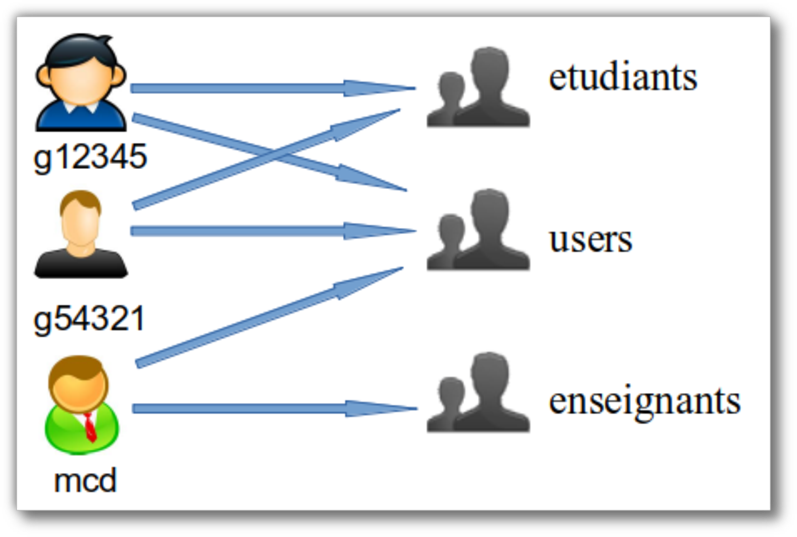
\includegraphics[width=.3\textwidth]{image/groupes.pdf}
			\vspace{-3em}
		\end{wrapfigure}
		\textbf{Exemple} :
		Dans l'exemple ci-contre on peut constater que :
		\begin{itemize}
		\item 
			l'utilisateur \samp{g12345} appartient 
			aux groupes \samp{users} et \samp{etudiants} ;
		\item 
			l'utilisateur \samp{g54321} appartient aux mêmes groupes ;
		\item 
			l'utilisateur \samp{mcd} appartient 
			aux groupes \samp{users} et \samp{enseignants}.
		\end{itemize}
		
		À quoi servent les groupes ? 
		À gérer les permissions. 
		On va pouvoir dire un truc du genre : 
		\og{}Seuls les professeurs peuvent voir le contenu de ce fichier\fg{}.

		\begin{theorie}{Visualiser les groupes}
			La commande \samp{groups} renseigne sur les groupes.
			\begin{itemize}
				\item \kbd{groups} : affiche les groupes de l'utilisateur.
				\item \kbd{groups loginUtilisateur} : affiche les groupes de l'utilisateur donné.
			\end{itemize}
			Le premier groupe de la liste est le \textbf{groupe principal}.
			C'est celui qui sera utilisé par défaut (par exemple, lorsqu'on crée un fichier).
		\end{theorie}

		\begin{Exercice}{Visualiser les groupes}
			\vspace{-1em}
			\begin{itemize}
				\item Visualiser les groupes auxquels vous appartenez.
				\item Quel est votre groupe principal ? 
				\item Quels sont les groupes auxquels appartient votre professeur ?
				\item Avez-vous un groupe en commun avec lui ?
				\item Quel(s) groupe(s) Linux avez-vous en commun avec les autres étudiants de votre groupe ÉSI ?
			\end{itemize}
		\end{Exercice}

		\begin{colxbox}[colback=white,drop fuzzy shadow]
			Les groupes qui existent concrètement sur une machine sont définis 
			par l'administrateur%
			\footnote{
				L'administrateur est la personne qui installe 
				un système d'exploitation et le gère au quotidien : 
				installation de logiciels, 
				gestion des comptes utilisateurs et des groupes, 
				sauvegardes, gestion des panne\dots{}
				Sur Linux, on dit aussi le « super user », 
				le « compte root » ou le « root ».
			} de la machine. 		
			Sur \texttt{linux1}, 
			il y a 3 groupes pour les utilisateurs.
			\begin{itemize}
				\item \textbf{\samp{users}} : tous les utilisateurs sont dans ce groupe
				\item \textbf{\samp{etudiants}} : tous les étudiants sont dans ce groupe
				\item \textbf{\samp{enseignants}} : tous les professeurs sont dans ce groupe	
			\end{itemize}
		\end{colxbox}

		\medskip
		\begin{alertbox}
			Attention, on remarque que vous confondez souvent 
			la notion de \textbf{groupe d'étudiants} à l'école
			et les \textbf{groupes sur Linux}.
			C'est un même mot qui recouvre 2 
			\textbf{concepts} complètement \textbf{différents}.
		\end{alertbox}

	%======================================
	\subsection{Propriétaire d'un fichier}
	%======================================
	
		\exergue{La propriété est un piège: ce que nous croyons posséder nous possède.}
			{Alphonse Karr}
		\vspace{2em}

		\exergue{La propriété c'est le vol.}{Pierre Joseph Proudhon}
		\vspace{1em}

		\begin{theorie}{Propriétaire}
			Chaque fichier/dossier \textbf{appartient} à une personne, 
			son \textbf{propriétaire}.
		\end{theorie}

		Pour visualiser le propriétaire d'un fichier, 
		on peut utiliser la commande \kbd{ls -l}.

		\begin{center}
			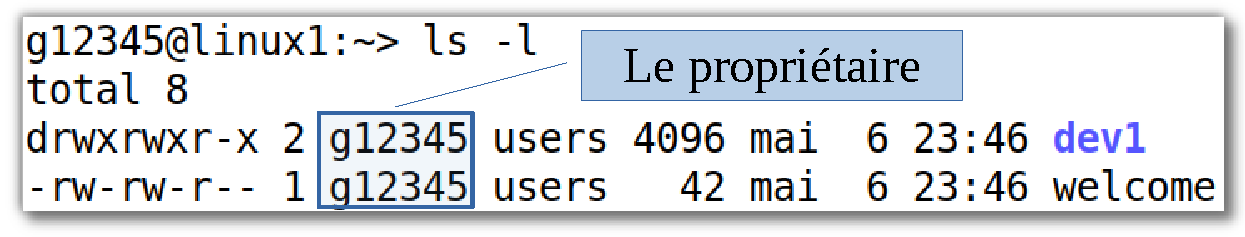
\includegraphics[height=5em]{image/owner}
		\end{center}

		On pourra donner des permissions spécifiques au propriétaire du fichier.

		\begin{Exercice}{Propriétaire}
			Visualisez le propriétaire des fichiers de votre dossier personnel.
		\end{Exercice}

		\begin{faq}
			\textbf{Les fichiers dans mon dossier personnel ne sont pas automatiquement à moi ?}

			Non. En pratique c'est généralement le cas, 
			mais on peut très bien trouver dans un dossier personnel 
			un fichier qui appartient à quelqu'un d'autre.  
		\end{faq}

	%======================================
	\subsection{Groupes d'un fichier}
	%======================================

		\begin{theorie}{Groupe d'un fichier}
			Chaque fichier/dossier \textbf{appartient} à \textbf{un et un seul groupe}.
		\end{theorie}

		\begin{center}
			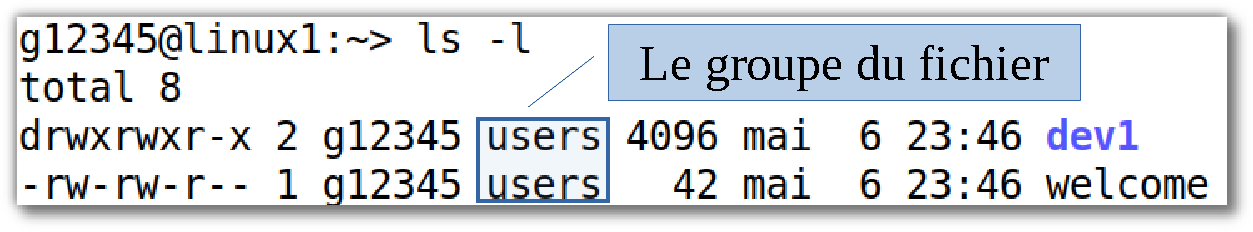
\includegraphics[height=5em]{image/group}
		\end{center}

		Ces groupes sont les mêmes que ceux utilisés pour grouper les utilisateurs.
		On pourra donner des permissions spécifiques à toutes les personnes
		qui sont dans le même groupe que le fichier.

		\begin{theorie}{Changer le groupe}
			\kbd{chgrp nouveauGroupe nomFichier}
			place le fichier indiqué dans le groupe donné.
		\end{theorie}

		Par défaut, un fichier est placé dans le groupe principal de celui qui le crée.

		\begin{Exercice}{Groupe}
			\vspace{-1em}
			\begin{itemize}
			\item Visualisez vos fichiers et déterminez à quel groupe ils appartiennent.
			\item Créez un fichier de test et modifiez le groupe auquel il appartient.
			\end{itemize}
		\end{Exercice}

	%======================================
	\subsection{Les 3 catégories de personnes}
	%======================================

		\begin{infotbox}{Ce qu'on a déjà vu}
			Un fichier a un propriétaire et appartient à un groupe.
		\end{infotbox}

		\begin{alerttbox}{Restez concentré !} 
			D'expérience nous constatons que vous avez du mal avec 
			les notions qui vont suivre.
			Restez concentrés et vérifiez que vous avez bien compris.
		\end{alerttbox}
		
		Lorsque nous allons donner des permissions sur un fichier/dossier,
		nous allons pouvoir donner des droits différents à trois catégories
		de personnes : le propriétaire, les utilisateurs qui sont dans le même
		groupe que le fichier et tous les \og{}autres\fg{} 
		(ceux qui ne sont pas dans les deux premières catégories).

		\begin{center}
			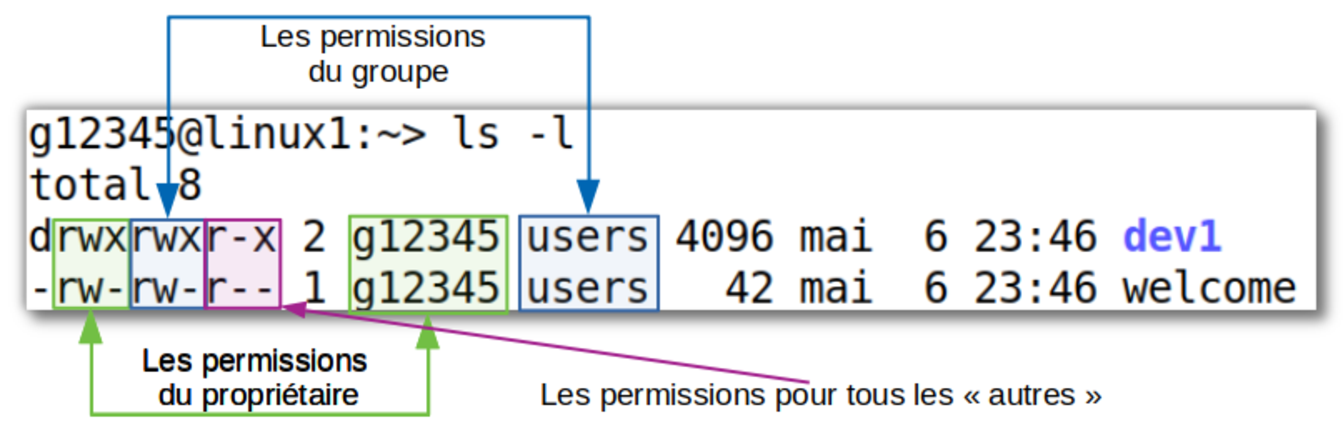
\includegraphics[width=.8\textwidth]{image/categorie}
		\end{center}

	%======================================
    \subsection{Les permissions sur un fichier}  
	%======================================

		Nous avons vu que nous pouvons spécifier des permissions différentes
		à trois catégories de personnes.
		Bien ! Mais quelles permissions pouvons-nous donner ?
		À quoi correspondent les lettres \samp{r}, \samp{w} et \samp{x}
		vues dans la capture d'écran précédente ?
		Commençons par les permissions pour un fichier.

		\begin{theorie}{Les permissions sur un fichier}
			Il existe 3 types de permissions pour un fichier : 
			lecture, écriture et exécution.
			\begin{description}
			\item[r (pour \emph{Read}, la lecture)] 
				Avec ce droit, un utilisateur peut 
				\emph{lire} un fichier, il peut en voir le contenu. 
				Par exemple, avec \samp{cat}.
			\item[w (pour \emph{Write}, l'écriture)]
				Un utilisateur a le droit en écriture sur un fichier, 
				il peut en modifier le contenu. 
				Par exemple, avec \samp{nano}.
			\item[x (pour \emph{eXecute}, l'exécution)]
				Cette permission concerne les exécutables. 
				Un exécutable est un fichier qui contient 
				un programme en langage machine 
				directement exécutable par le processeur.
				Par exemple, il existe quelque part sur le disque 
				un fichier \samp{nano} 
				qui contient le programme de la commande nano.
			\end{description}
		\end{theorie}

		Les permissions sont toujours placées dans le même ordre (\samp{rwx})
		et un tiret (\samp{-}) indique que la permission n'est pas accordée.

		\paragraph{Exemple.}
		Reprenons la capture d'écran précédente et interprétons
		les permissions sur le fichier \samp{welcome}.
		\begin{center}
			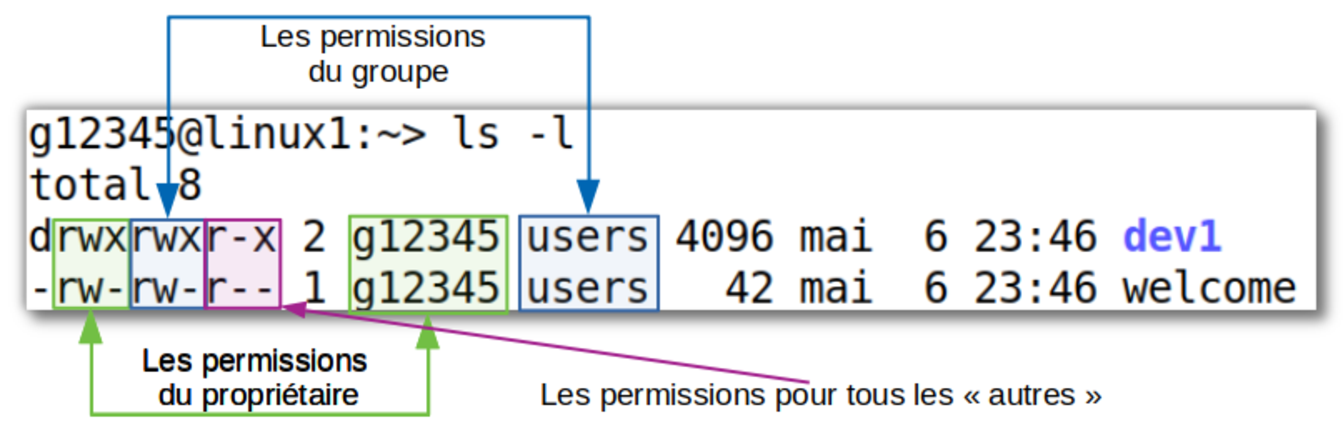
\includegraphics[width=.8\textwidth]{image/categorie}
		\end{center}
		On y lit que :
		\begin{itemize}
		\item
			Les permissions pour le propriétaire sont \samp{rw-}.
			Donc, (\samp{g12345}) 
			peut voir \textbf{(r)} le contenu 
			et modifier \textbf{(w)} le fichier \samp{welcome}.
			Par contre, il ne peut pas l'exécuter.
		\item 
			Idem pour les utilisateurs qui sont dans le groupe \samp{users}.
		\item 
			Les autres utilisateurs 
			(ceux qui ne sont ni le propriétaire, ni un utilisateur du groupe \samp{users})
			peuvent lire le fichier mais pas le modifier ni l'exécuter.
		\end{itemize}

		\medskip
		\begin{Exercice}{Déterminez les bonnes permissions}
			Imaginons que vous écrivez un programme \name{Java} sur \texttt{linux1}.
			Vous ne voulez pas que quelqu'un copie sur vous.
			Par contre, vous désirez qu'il puisse exécuter la version compilée.
			Quelles permissions proposez-vous pour les fichiers :
			\begin{itemize}
			\item \samp{.java} ? 
				{\tiny
					\textfield{r}\textfield{w}\textfield{-}\quad
					\textfield{-}\textfield{-}\textfield{-}\quad
					\textfield{-}\textfield{-}\textfield{-}
				}
			\item \samp{.class} ? 
				{\tiny
					\textfield{r}\textfield{-}\textfield{-}\quad
					\textfield{r}\textfield{-}\textfield{-}\quad
					\textfield{r}\textfield{-}\textfield{-}
				}
			\end{itemize}
		\end{Exercice}

		\begin{Experience}{Permissions par défaut}
			Quelle est la situation de départ quand on crée un fichier ?
			Faisons une petite expérience pour le découvrir.
			\begin{steps}
			\item Si ce n'est pas encore fait, créez un dossier \samp{dev1/td2}.
			\item Créez-y un fichier vide.
			\item Demandez les détails du fichier (propriétaire, groupe, permission)
			\end{steps}
			On constate qu'un nouveau fichier appartient à celui qui l'a créé 
			(on s'en doute) et au groupe principal du créateur. 
			Il y a aussi des permissions par défaut (plutôt permissives dans notre cas).  
		\end{Experience}		
	
	%=========================================
	\subsection{Modifier les permissions}
	%=========================================

		\begin{infotbox}{Faisons le point !}
			Nous savons qu'un fichier a un propriétaire et un groupe.
			Nous savons que nous allons pouvoir donner des permissions
			différentes au propriétaire, au membres du groupe 
			et à tous les autres utilisateurs.
			Nous avons aussi appris à comprendre les permissions données sur un fichier.
		\end{infotbox}
	
		Très bien mais comment modifier ces permissions ?

		\begin{theorie}{Modifier les permissions}
			\kbd{chmod permissions fichier} modifie les permissions du fichier.
		\end{theorie}

		Il existe deux façons d'indiquer les permissions : via des nombres ou via des lettres.

		\subsubsection{Donner les permissions avec des nombres}
		%======================================================

			Pour indiquer les permissions avec un nombre, 
			on considère que $r=4$, $w=2$ et $x=1$. 
			Et on additionne les valeurs ainsi obtenues.

			Exemples :
			\begin{tabular}{|c|c|l|}
				\hline
				\textbf{lettres} & \textbf{nombre} & \textbf{signification}\\
				\hline
				\samp{r-{}-} & 4 (4+0+0) & droit en lecture uniquement\\
				\samp{rw-}   & 6 (4+2+0) & droit en lecture et en écriture\\
				\samp{-{}-x} & 1 (0+0+1) & droit d'exécution uniquement\\
				\hline
			\end{tabular}

			On combine alors les nombres obtenus pour les 3 sortes d'utilisateurs.
			
			Exemple : \kbd{chmod 640 welcome} donne 
			au propriétaire le droit en lecture/écriture, 
			aux utilisateurs dans le même groupe que le fichier le droit en lecture uniquement 
			et aucun droit aux autres.

			\begin{Exercice}{Convertir les permissions en nombres} 
				Reprenez les permissions affichées dans la capture d'écran ci-dessous 
				et exprimez-les avec un nombre de 3 chiffres.  
				\begin{center}
					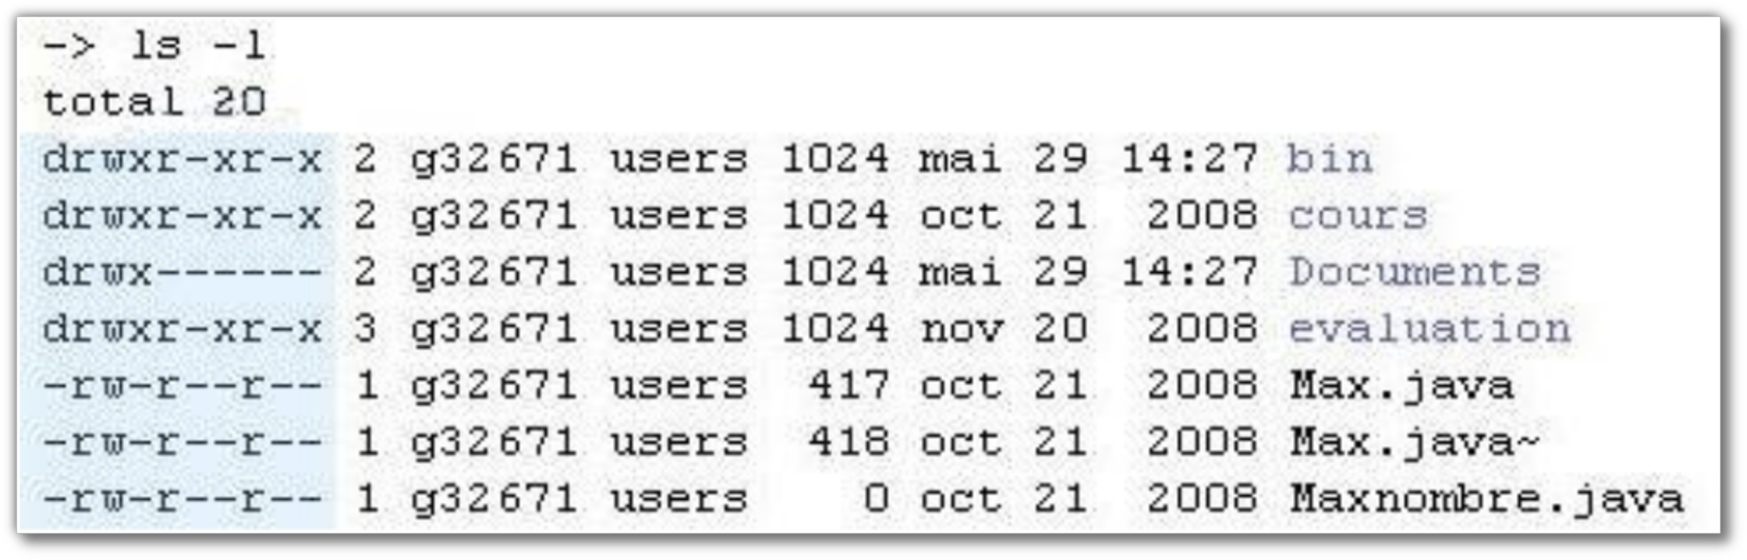
\includegraphics[width=0.7\linewidth]{image/perm-nb.pdf}
				\end{center}
			\end{Exercice}
			
			\begin{Exercice}{Modifier les permissions}
				Créez un fichier \samp{dev1/td2/brol} 
				contenant un petit texte de votre choix.
				Faites en sorte qu'il soit lisible par tout le monde
				mais modifiable uniquement par vous.
			\end{Exercice}

		\subsubsection{Donner les permissions avec des lettres}
		%======================================================

			Avec la notation précédente, on spécifie toutes les permissions. 
			Ici, on va aussi pouvoir indiquer uniquement ce qui doit changer : 
			ajouter/enlever un droit sans toucher aux autres droits.

			\begin{wrapfigure}{r}{.4\textwidth}
				\vspace{-1em}
				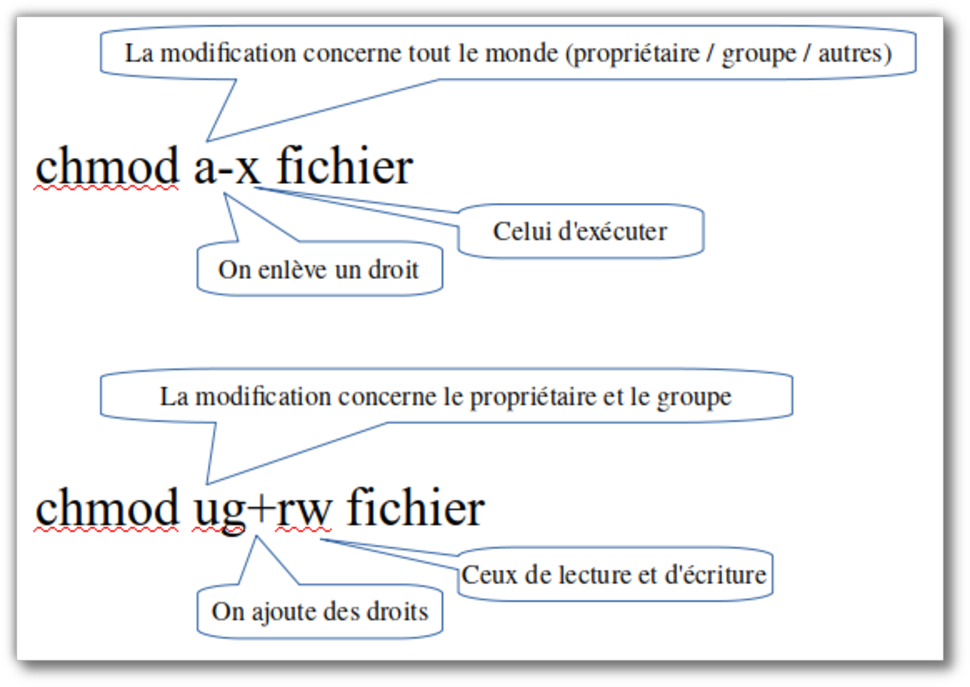
\includegraphics[width=.4\textwidth]{image/chmod.pdf}
				\vspace{-2em}
			\end{wrapfigure}
			Le format de la commande est assez complexe. 
			\begin{itemize}
			\item
				On indique d'abord les utilisateurs concernés par la modification des droits :
				\begin{itemize}
				\item « u » pour le propriétaire (user), 
				\item « g » pour le groupe, 
				\item « o » pour les autres (other) et
				\item « a » pour tout le monde (all)
				\end{itemize}  
			\item
				On indique ensuite si on veut ajouter (« + ») 
				ou enlever (« - ») un droit
			\item 
				On indique enfin quel(s) droit(s) on ajoute ou enlève 
				(« r », « w » et/ou « x »)
			\end{itemize}

			Consultez à la page de manuel pour découvrir toutes les possibilités.

			\begin{Exercice}{Modifier les permissions}
				Créez un fichier \samp{dev1/td2/brol2} 
				contenant un petit texte de votre choix.
				Faites en sorte qu'il soit lisible par tout le monde
				mais modifiable uniquement par vous.
			\end{Exercice}

	%======================================================
	\subsection{Différencier les étudiants des enseignants}
	%======================================================

		\begin{alertbox}
			Nous n'allons pas ici introduire un concept nouveau
			mais appliquer tout ce qui a été vu dans un exemple
			qui, par expérience, vous pose souvent un problème. 
		\end{alertbox}

		\begin{Tutoriel}{Droit de lecture pour les enseignant uniquement}
			Supposons que vous avez un fichier qui ne doit être
			lu que par vous-même et les enseignants (mais pas les autres étudiants).

			Comment donner des droits différents aux enseignants et aux étudiants ?
			La seule solution passe par une modification du groupe du fichier.
			S'il appartient au groupe \samp{etudiants} par exemple
			et plus au groupe \samp{users}, les permissions de groupe
			s'appliqueront aux étudiants et les permissions des \emph{autres}
			concerneront les enseignants%
			\footnote{
				Pour être plus précis, 
				tout utilisateur qui n'est pas dans le groupe \samp{etudiants}.
			}

			\begin{steps}
			\item 
				Entrez \kbd{cd ~/dev1/td2}
				pour vous placer dans le dossier indiqué.
			\item 
				Entrez \kbd{touch examen} 
				pour créer le fichier (vide) indiqué.
			\item 
				Entrez \kbd{chgrp etudiants examen}
				pour changer son groupe.
			\item 
				Entrez \kbd{ls -l} pour visualiser la modification.
			\item 
				Entrez \kbd{chmod 604 examen}
				pour changer les permissions associées au fichier.
			\item 
				Entrez \kbd{ls -l} pour visualiser le résultat final.
			\end{steps}
		\end{Tutoriel}

		\begin{Exercice}{Un fichier réservé aux étudiants}
			Créez un fichier \samp{dev1/td2/gossip}
			pour partager des rumeurs entre élèves.
			On voudrait que tous les étudiants puissent le lire et le modifier
			mais que les enseignants ne puissent ni le lire, ni l'écrire.
		\end{Exercice}

	%======================================================
	\subsection{Les permissions sur les dossiers}
	%======================================================

		\begin{wrapfigure}{r}{.2\textwidth}
			\vspace{-1em}
			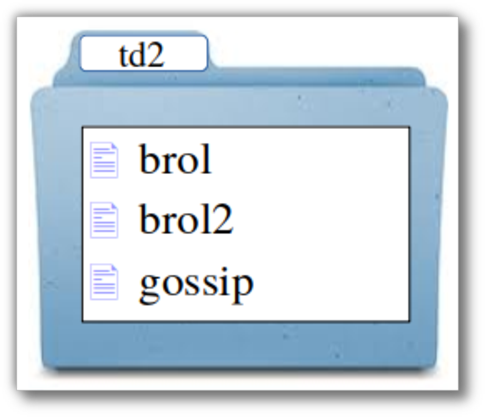
\includegraphics[width=.2\textwidth]{image/perm-dossier.pdf}
			\vspace{-4em}
		\end{wrapfigure}
		Tout comme pour les fichiers, on peut donner des permissions au dossier. 
		Ce qui change, c'est la signification des permissions. 
		Que veut dire « exécuter » un dossier par exemple ? 
		
		Pour bien comprendre, prenons une image.
		Imaginons qu'un dossier possède sur sa « couverture » une liste de son contenu. 
		Par exemple, on voit ci-contre que le dossier td2 contient 3 fichiers.
		
		\begin{theorie}{Permissions sur un dossier}
			Explicitons à présent le sens de chaque droit pour un dossier :
			\begin{description}
			\item[\samp{r} (lecture)] 
				On a le droit de lire ce qui est écrit sur la « couverture » du dossier. 
				On peut par exemple faire \kbd{ls td2}.
			\item[\samp{w} (écriture)] 
				On peut modifier la « couverture » du dossier. 
				On peut ainsi effacer un fichier (\kbd{rm td1/brol2})
				ou en créer un (\kbd{touch td1/brol3}). 
			\item[\samp{x} (ouverture)]
				On peut « ouvrir » le dossier / entrer dedans. 
				On peut ainsi en faire son dossier courant (\kbd{cd td2}) 
				ou le traverser dans un chemin (\kbd{cat td2/gossip}).				
			\end{description}
		\end{theorie}

		\begin{alertbox}
			Pour effacer un fichier 
			il ne faut pas de droit en écriture sur le fichier 
			mais bien sur le dossier qui le contient.
		\end{alertbox}
		
		\begin{Exercice}{Les permissions sur un dossier (I)}           
			Dans un dossier \samp{dir1} dans votre dossier \samp{td2}.
			Dans ce dossier, créez un fichier \samp{file}.
			Faites en sorte que tout le monde puisse voir 
			quels fichiers se trouvent dans \samp{dir1}
			mais sans pouvoir lire le contenu de ces fichiers.
		\end{Exercice}

		\begin{Exercice}{Les permissions sur un dossier (II)}           
			Dans un dossier \samp{dir2} dans votre dossier \samp{td2}.
			Dans ce dossier, créez un fichier \samp{file}.
			Faites en sorte que tout le monde puisse modifier ce fichier 
			mais sans pouvoir le supprimer.
		\end{Exercice}

	%================================
	\subsection{Les derniers détails}
	%================================

		Voyons quelques détails mis de coté pendant notre apprentissage.

		\begin{center}
			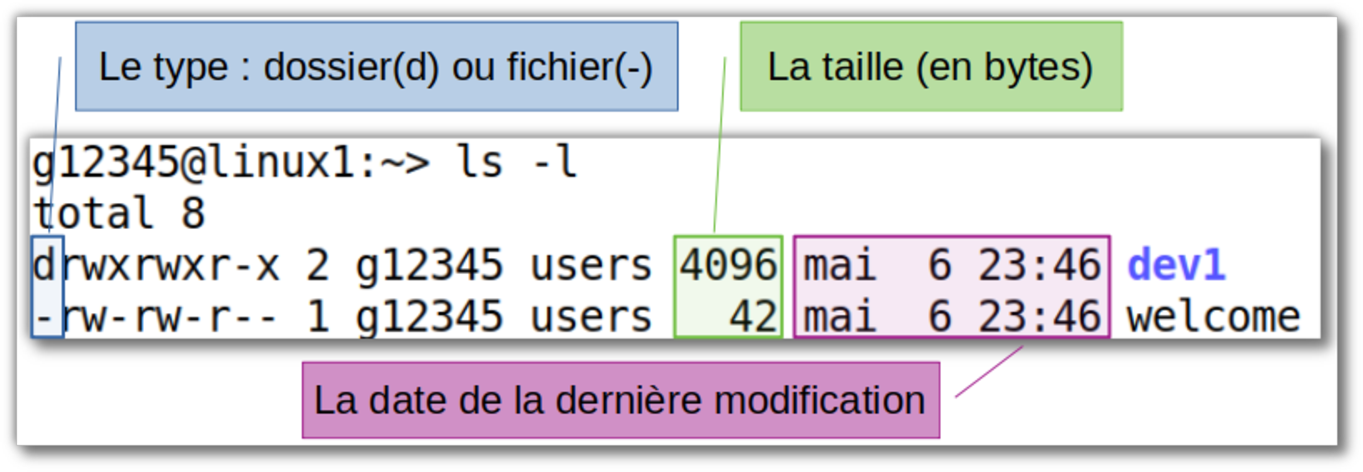
\includegraphics[width=.7\textwidth]{image/reste.pdf}
		\end{center}

		\begin{faq}
			\textbf{%
				Vous dites que dans un affichage en format long, 
				le premier caractère indique si c'est un fichier simple ('-') ou un dossier ('d'). 
				Pourtant j'ai déjà vu d'autres symboles. C'était quoi ?
			}
			
			Il existe d'autres types de fichiers que les deux que nous avons vus. 
			Ils se rencontrent moins souvent et sont surtout utilisés par le système.
			Par exemple, certains définissent des \textit{pilotes} vers le matériel. 
			Si vous voulez en savoir plus, vous pouvez lire ceci 
			(\url{en.wikipedia.org/wiki/Unix\_file\_types}).  

			\medskip
			\textbf{%
				Vous avez mentionné les permissions 'r', 'w' et 'x'. 
				Pourtant j'ai déjà vu d'autres lettres dans la zone réservée aux permissions. 
				C'était quoi ?
			}

			Il y a 3 permissions dont nous n'avons pas parlé parce qu'elles sont moins courantes : 
			le \textit{suid} (set user id), le \textit{sgid} (set group id) 
			et le \textit{sticky}. 
			Si vous voulez en savoir plus, vous pouvez lire ceci 
			(\url{fr.wikipedia.org/wiki/Permissions\_UNIX}).  

			\medskip
			\textbf{%
				J'ai un Linux à la maison et les groupes ne sont pas les mêmes. 
				C'est normal ?
			}

			Oui ! 
			Les groupes dépendent à la fois de la distribution particulière utilisée
			et de la façon dont l'administrateur (le root) a configuré le système.   

			\medskip
			\textbf{%
				Vous n'avez pas expliqué le sens de la 2\ieme{} colonne 
				fournie par la commande ls (juste avant le propriétaire) ?
			}

			C'est vrai mais c'est moins utile 
			et plus lié à la structure interne du système de fichier. 
			Je veux bien vous dire qu'il s'agit 
			du nombre de liens physiques sur le fichier 
			mais je sens que vous commencez déjà à regretter d'avoir posé la question ;)  

			\medskip
			\textbf{%
				Nous avons vu qu'un fichier est créé avec des permissions par défaut. 
				C'est configurable ?
			}

			Oui. Voyez la commande \kbd{umask}.  
		\end{faq}

%===================
\section{Conclusion}
%====================

	\begin{theorie}{Notions importantes de ce TD}
		Voici les notions importantes que vous devez avoir assimilées à la fin de ce TD.
		\begin{itemize}
		\item 
			Comprendre que les utilisateurs sont placés dans des groupes.
		\item 
			Pouvoir visualiser le propriétaire d'une fichier.
		\item 
			Pouvoir visualiser/modifier le groupe d'un fichier.
		\item 
			Comprendre comment fonctionnent les permissions
			(lecture, écriture, exécution et les 3 catégories de personnes).
		\item 
			Pouvoir visualiser les permissions
			et les modifier (en utilisant des lettres et des nombres).
		\item 
			Comprendre ce qu'il y a de spécifique en ce qui concerne les permissions
			sur les dossiers.
		\end{itemize}
	\end{theorie}

\end{document}
